% !TeX root = ../main.tex

\chapter{石墨烯的制备、表征}

\section{石墨烯的早期制备}

在石墨烯的早期发展上,率先被制备出来的是\textit{氧化石墨}和\textit{氧化石墨烯},伴随着后面本杰明·柯林斯·布罗迪对实验方法的改进,以及吕斯、沃格特、汉斯勃姆等人的研究,确认了氧化石墨烯在稀碱性介质中与肼、硫化氢或二价铁盐中会发生氧化还原反应,生成薄层状的碳。

但是早期制取石墨烯的过程并不特别成功。1999年,罗德尼·鲁夫带领的团队曾经尝试过利用硅片摩擦的办法制备石墨烯,虽然我们现在已经知道,这样的办法产物中能得到少层、和极少量单层石墨烯,但鲁夫并没有对产物做进一步的研究,错过了发现石墨烯的机会。

荷兰物理学家赫勒采用了外延生长法的办法制备石墨烯,在2004年,他们的团队独立地利用碳化硅合成了石墨烯,并完成了单层石墨烯电学性质的测定,并发现了超薄外延石墨薄膜的二维电子气特性。但遗憾的是,赫勒并没有因此得到诺贝尔奖,但他的开拓性的工作值得被认可。

在同一年,盖姆团队利用了一种简单的胶带分离的办法制备了近乎完美的石墨烯,这是第一次严格意义上单层原子厚度的石墨烯的发现,他们检测出石墨烯独特的电学性质,掀起了全世界研究石墨烯的热潮。

如同诺奖委员会所说的那样,“石墨烯研究的难点并不在于制备出石墨烯的结构,而是分离出足够大、单个的石墨烯来确认、表征、验证石墨烯的性质”,对于盖姆来说,利用透明胶带离析技术是重要一步,但重要一步是希望能够找到石墨烯令人惊奇的物理性质。最终在盖姆的学生诺沃肖洛夫的耐心下,他们发现石墨烯碎片有着高度导电的性质。

同年,他们在\textit{Science}上发表了一篇具有里程碑意义的论文:\textit{Electric Field Effect in Atomically Thin Carbon Films},这篇论文率先描述了单晶石墨薄膜能够在普通环境下稳定存在、并且具有高度导电的性质,打破了各种方法研究石墨烯单层都没有进展的僵局,推翻了几十年来二维晶体不能稳定存在的预言。

\section{石墨烯的一般制备方法}

\subsection{物理方法}

\subsubsection{微机械剥离法}

以高温热解石墨为原料,在石墨片上刻蚀出一个平台,并涂上一层光刻胶。焙固后,平台面附着在光刻胶层上,从石墨片上剥离下来。留在光刻胶中的石墨可以利用丙酮释放出来,在溶液中插入硅片,得益于硅片和一些石墨烯薄片之间较强的范德华力,一些石墨薄片便会附着在硅片上。

这种方法费时费力、难以精确控制、重复性差、难以大规模制备。

\subsubsection{印章切取法}

在印章突起的表面上涂一层转换层,并按压在石墨上,高压下印章边缘将产生极大的剪切应力,使得石墨烯层从石墨上分离下来。类似地,可以制作“固定层”,将石墨烯从印章上剥落下来。

这种方法操作简单,但一般得到的多是四层石墨烯,难以制备单层石墨烯。

\subsection{化学方法}

\subsubsection{自上而下的合成方法}

石墨烯的化学制备方法是研究较早的方法,主要是以苯环或者其他芳香环为核,通过偶联反应使得苯环上的碳全部被取代,相邻取代基通过脱氢的方式形成新的芳香环,多步反应后是苯香体系变大。但面积较大的时候需要较多的催化剂,反应时间长,这种方法一般不能合成具有较大平面结构的石墨烯。

早期的合成方法是采取多环芳烃\textit{PAH}进行合成,但产率较低;经过改进后的这种方法主要是通过\textit{Diels-Alder}反应、Pd催化的\textit{Hagihara-Sonogashira},\textit{Buchwald-Hartwig}或\textit{Kumada/Negishi}偶合,先合成六苯并蔻\textit{HBC},然后在 $\ce{FeCl_3}$ 或 $\ce{Cu(OTf)_2-AlCl_3}$ 作用下环化脱氢,得到较大平面的石墨烯。\cite{RN2}

\begin{figure}
    \centering
    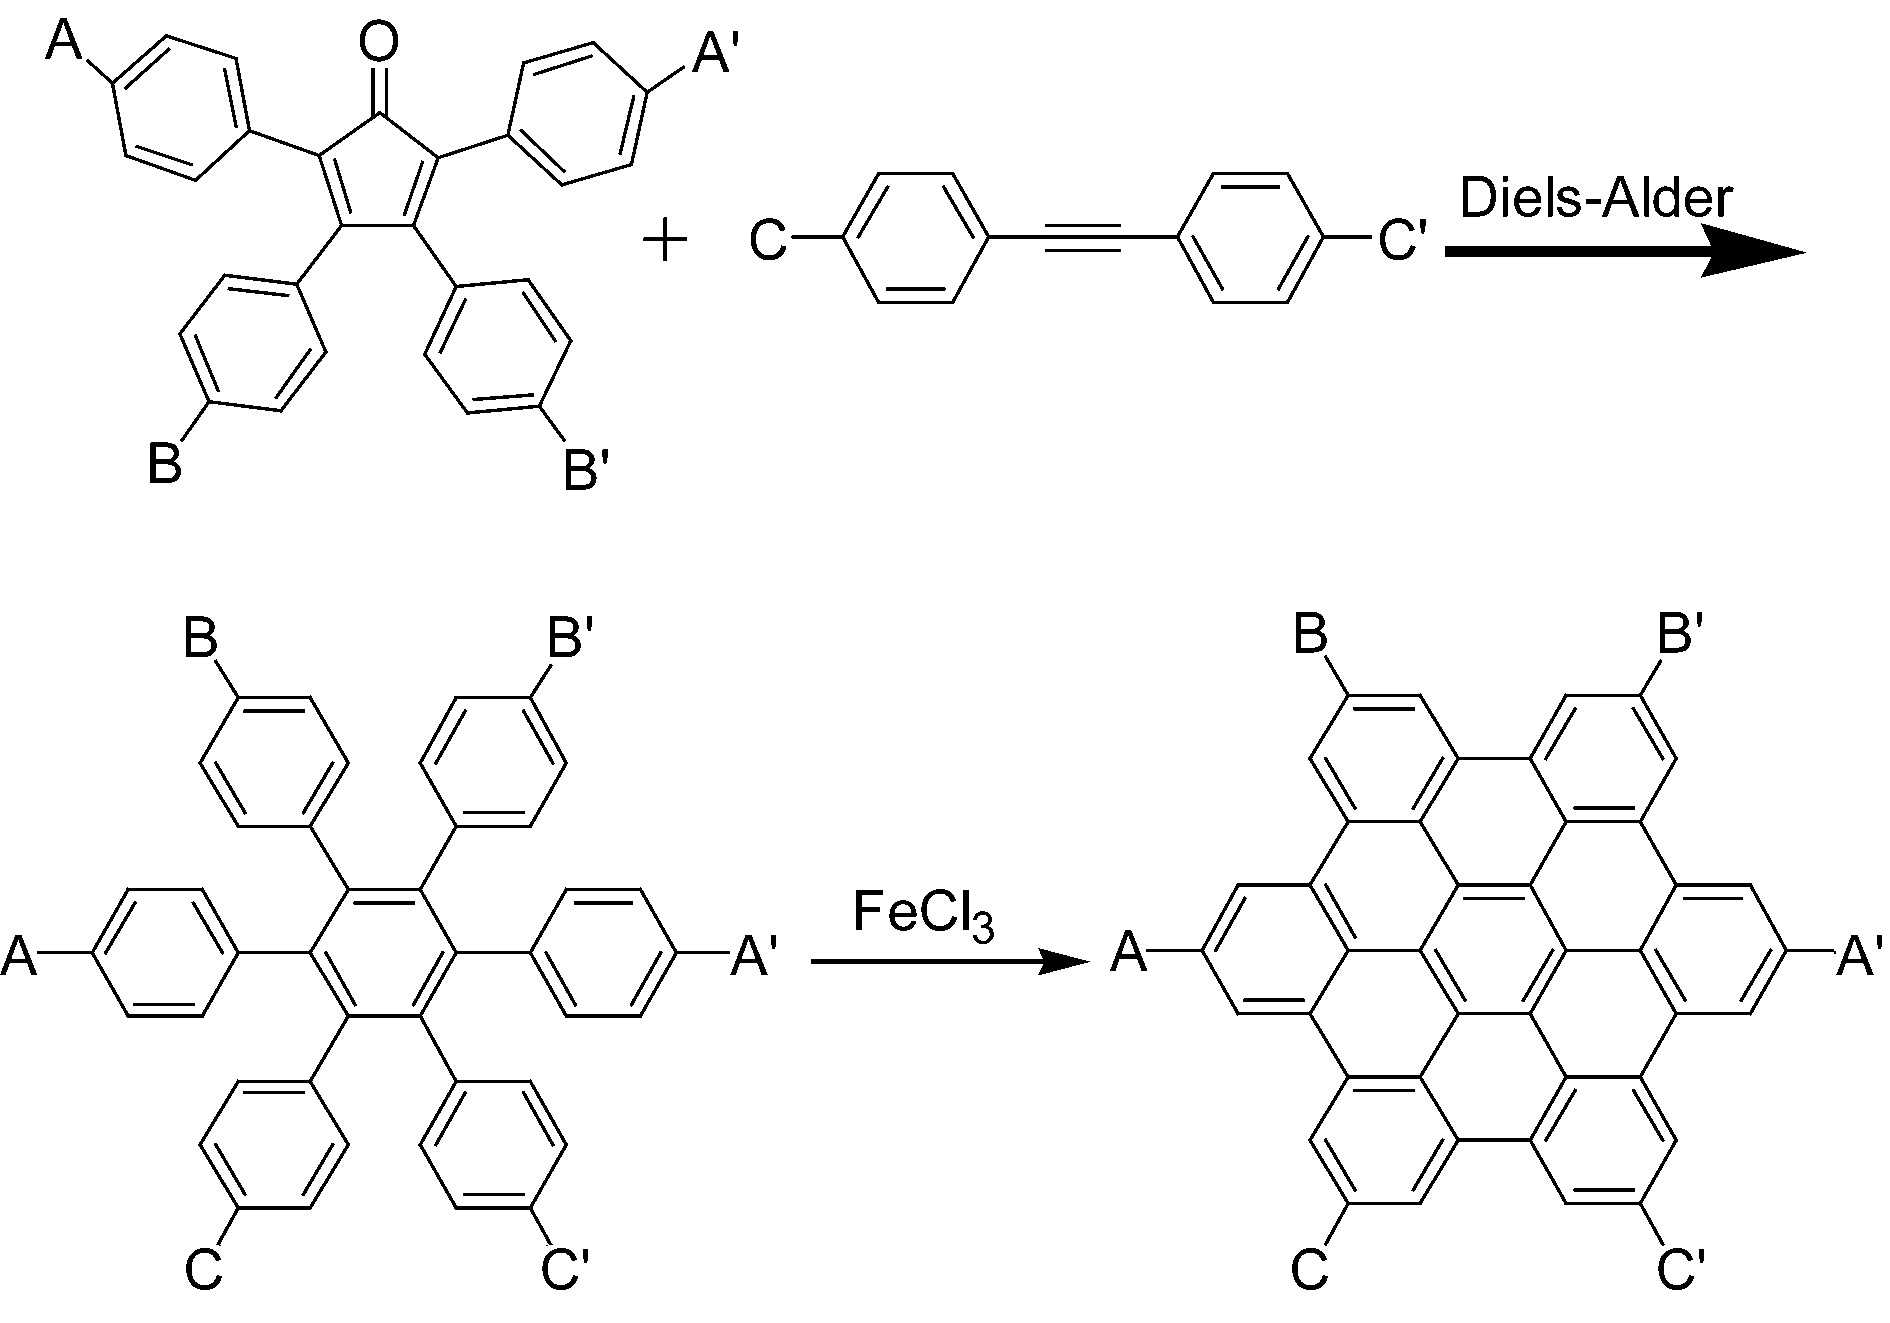
\includegraphics[scale=1.0]{img/production1}
    \caption{低对称HBC通用合成路线}
\end{figure}

\begin{figure}
    \centering
    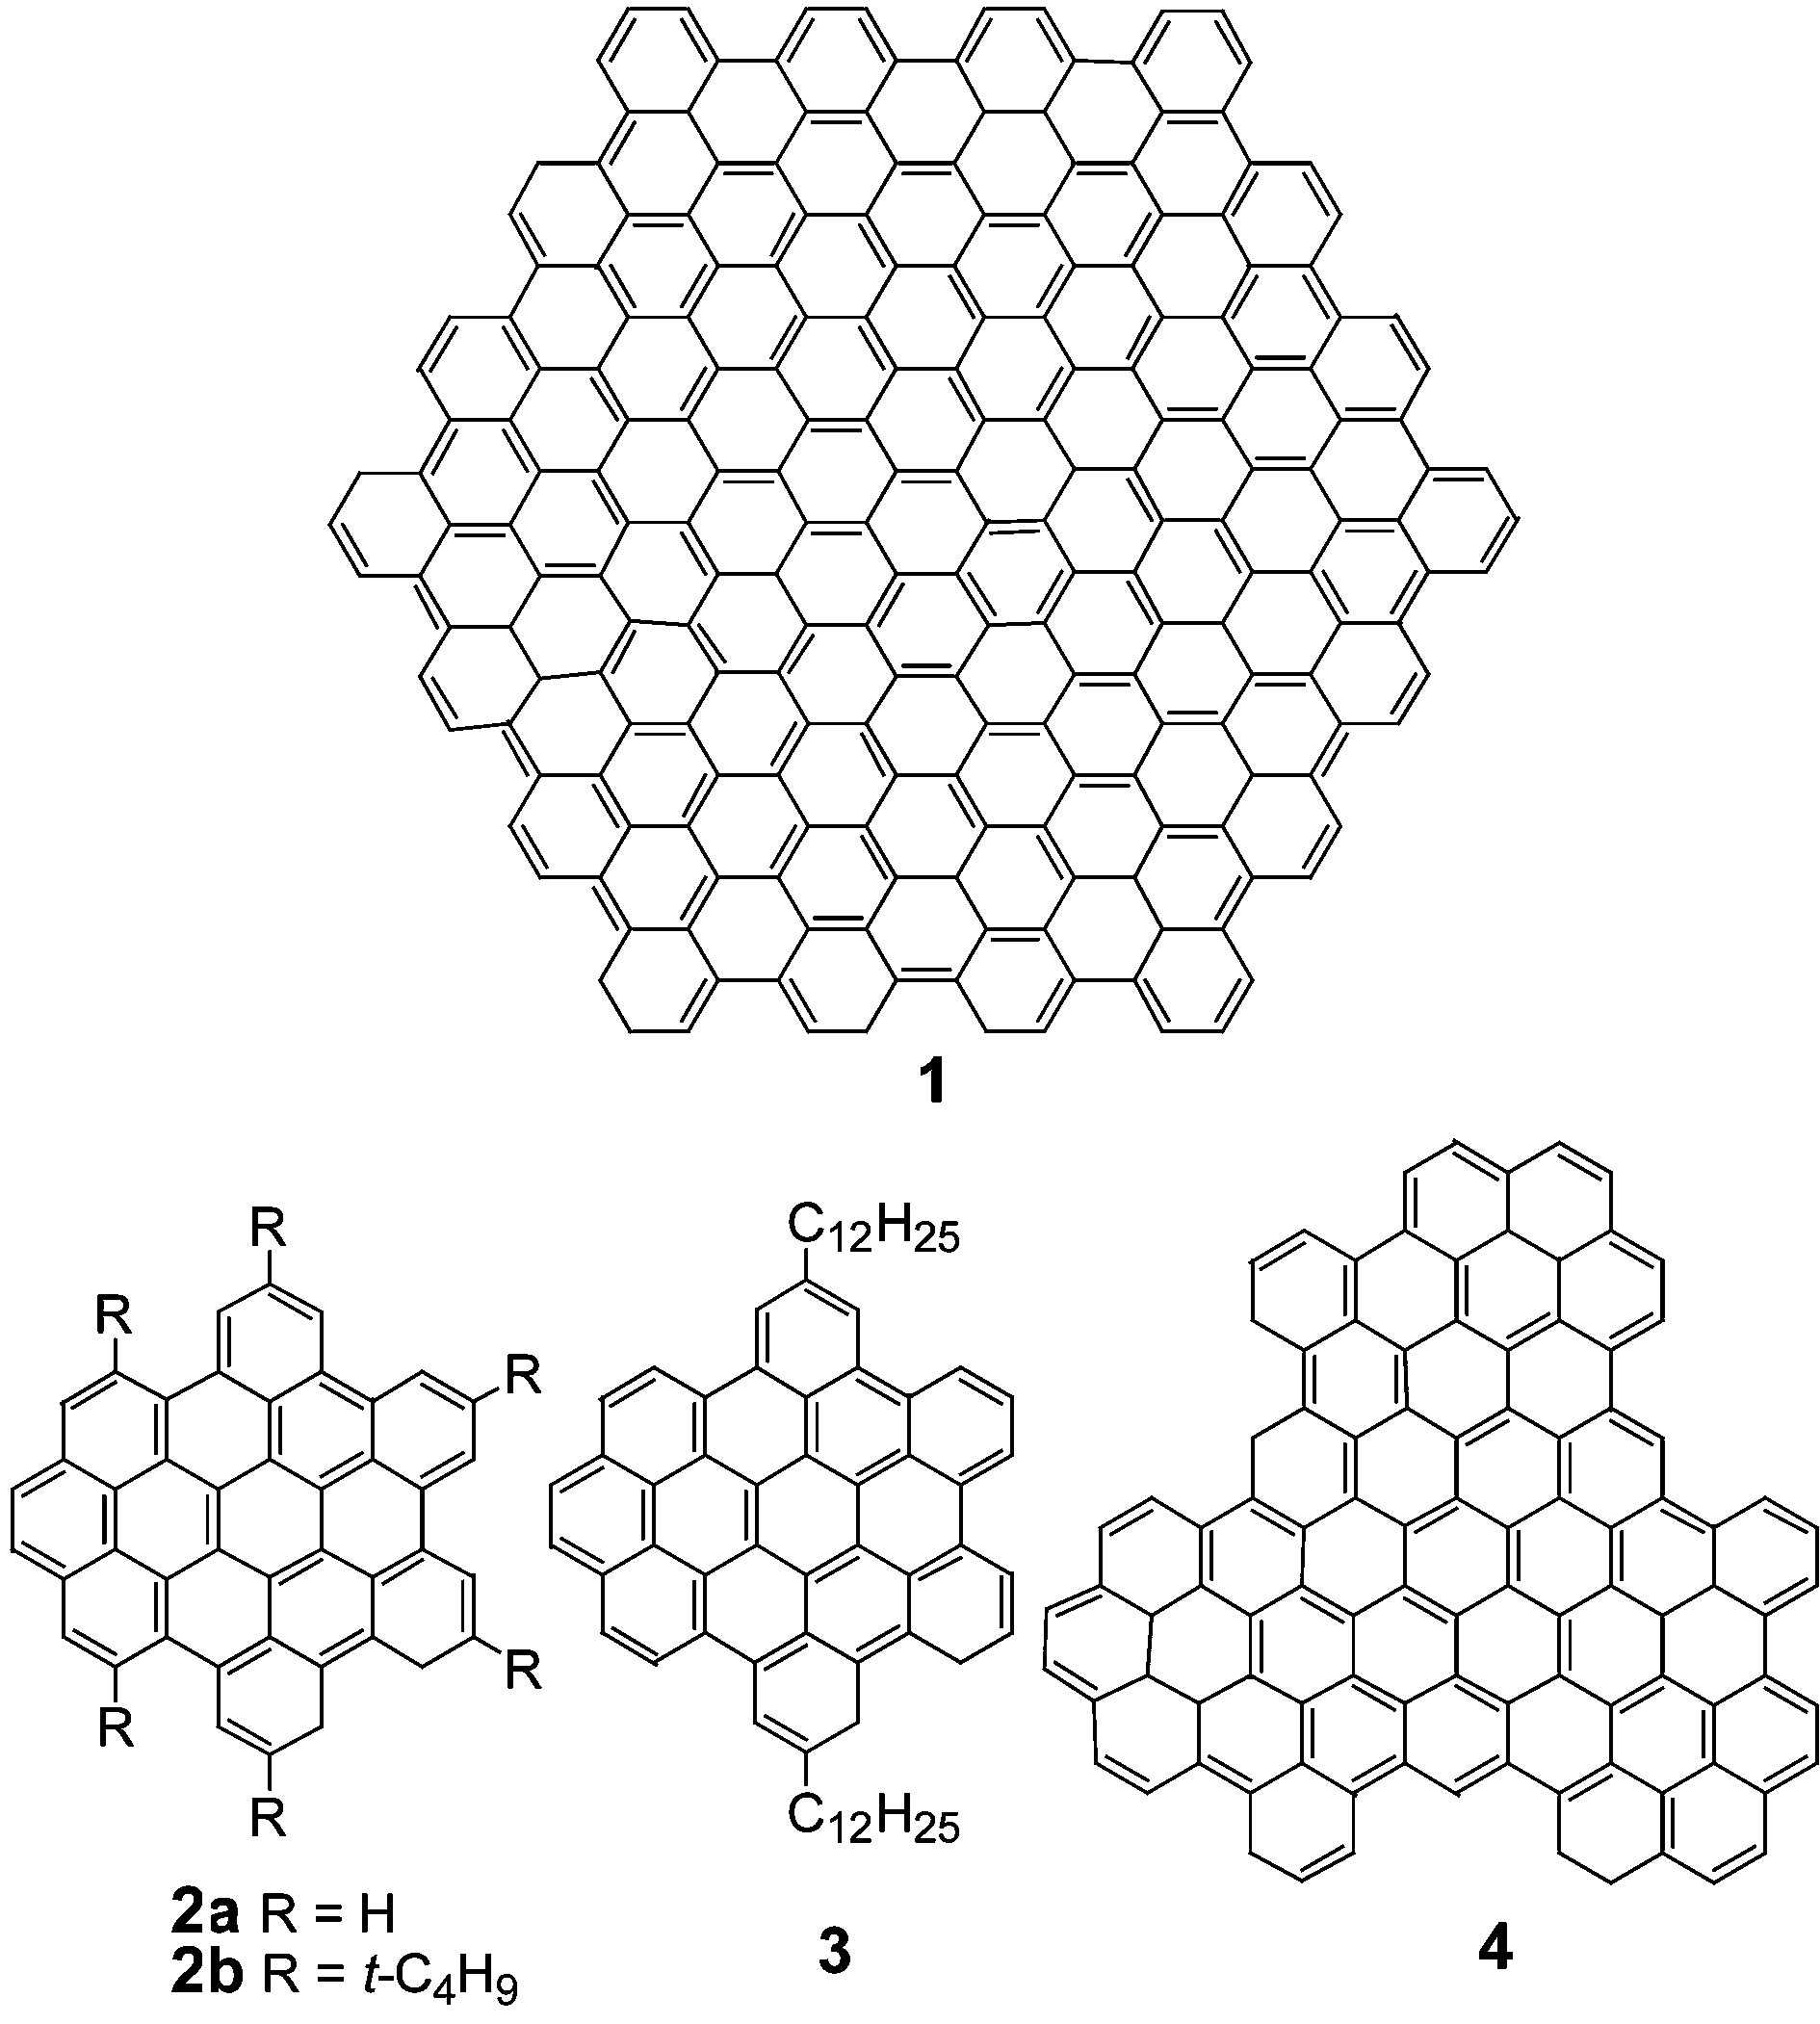
\includegraphics[scale=1.0]{img/production2}
    \caption{锯齿状石墨烯结构}
\end{figure}

这种方法的缺点是:反应步骤较多、时间长、脱氢效率不高,合成\textit{HBC}时,需要使用金属催化剂,会产生环境污染,一种改进的方法是通过乙醇和钠作原料,通过溶剂热法,可以制备以克为量级的石墨烯,产率更高,并且解决了环境污染问题。

\subsubsection{热解法}

这种方法以石墨为原材料,首先对表面进行氧化处理,然后再真空条件下加热到$1000^\circ C$,去除氧化物,去除后继续加热至$1250\sim 1450^\circ C$,形成石墨烯层,厚度与加热温度相关。

这种办法可以得到单层和双层石墨烯,但缺点同时也在于成膜不均匀,且对于条件要求过于严格,难以大规模制备。

\subsubsection{CVD 化学气相沉积法}

\textit{CVD},化学气相沉积,是一种利用反应物在相当高的温度、气态条件下发生化学反应,生成的固态物质沉积在加热的固态基体表面,进而制得固体材料的工艺技术。使用乙醇液滴作为碳源,利用Ar等离子体进行石墨烯的合成,可以极大地缩短反应时间。

\subsubsection{氧化—分散—还原法}

该方法是目前应用最广泛的合成方法,首先将石墨氧化,得到溶液中分散的石墨前体,最终利用还原剂得到单层或多层石墨烯。

这种方法中常用的氧化剂包括:$\ce{HNO_3}$(发烟)、$\ce{KClO_3}$、浓硫酸等,常用的还原剂有:水合肼、$\ce{NaBH_4}$、对苯二酚等。

为更彻底的破坏石墨烯层之间的范德华力,目前最常用的办法是对氧化石墨烯再进行修饰,最终还原,即氧化-修饰-还原的方法,常用的化学修饰方法为:共价键修饰、非共价键修饰和金属颗粒修饰。

尽管上述方法均能得到单层或者多层的石墨烯,但合成产率不高,且多数情况下不能得到单层的结构。目前石墨烯合成的办法已经取得初步的成效,但仍然是研究的重要任务之一。


\section{石墨烯的表征}

石墨烯的表征,主要分为图像类和图谱类\cite{RN11}。图像类包括光学显微镜、扫描电子显微镜、透射电子显微镜、原子力显微镜等,图谱类包括拉曼光谱、红外光谱、X射线光电子能谱、紫外光谱等。下面我们具体介绍。

\subsection{光学显微镜表征}

光学显微镜可用于快速表征石墨烯层数。使用涂有氧化物的硅片作衬底,由于衬底和石墨烯对特定光的反射光强不同,会观察到颜色和对比度的差异,借此分辨层数\cite{RN12}。

光学显微镜对石墨烯层数的表征直观快捷,但是往往只能区分单层石墨烯和多层石墨烯,无法精确分辨石墨烯的层数。

\subsection{扫描电子显微镜(SEM)表征}

通过SEM图像的颜色和表面褶皱可以大致判断出石墨烯的层数。随着石墨烯层数增大,褶皱程度越来越小,颜色越来越深。

SEM对石墨烯层数的表征和光学显微镜相似,仍不够精细。

\subsection{透射电子显微镜(TEM)表征}

利用TEM,观察石墨烯边缘或褶皱处的显微像,可以简单估计石墨烯的层数和尺寸,当然这较为粗略。

不过,相较于光学显微镜和SEM,TEM可以更精确地表征石墨烯的层数。根据透射电镜中电子衍射的原理,改变电子束入射方向时,单层石墨烯的各衍射斑的强度几乎不变,而多层石墨烯则有明显改变,由此可以判断层数\cite{RN12}。然而,此方法仍有局限性,只适用于大块样品。

\subsection{原子力显微镜(AFM)表征}

原子探针接近样品表面到一定距离时,原子间作用力迅速上升,因而根据探针受力的大小可以分析样品表面的形貌特征。特别地,对于石墨烯,AFM可表征石墨烯的横向尺寸、面积和厚度等。

通过AFM,我们可以表征氧化石墨烯的还原过程。将氧化石墨烯用蔗糖溶液还原过程前后的AFM图像如图~\ref{fig:AFM}\cite{RN13}:

\begin{figure}
    \centering
    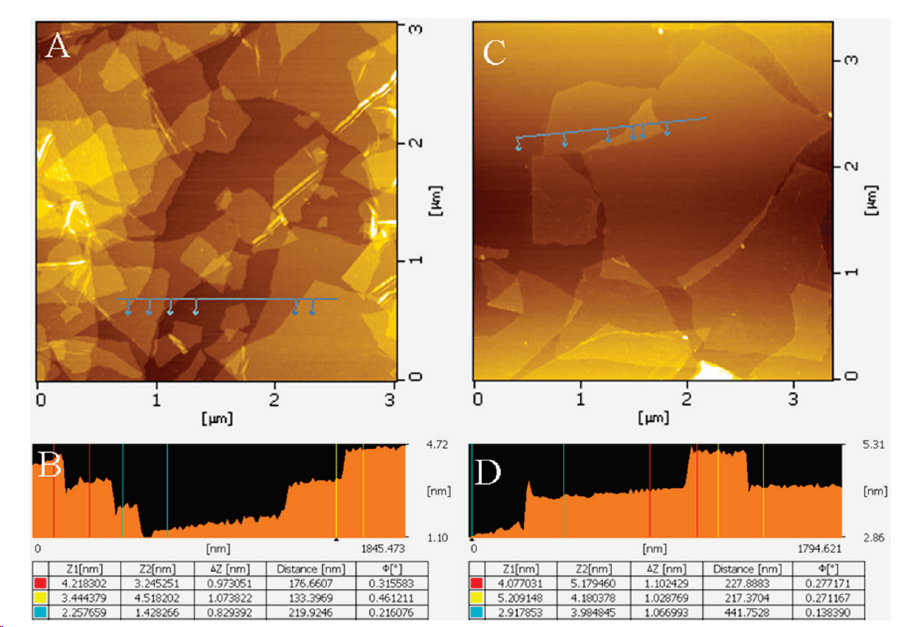
\includegraphics[scale=0.4]{img/AFM}
    \caption{石墨烯AFM图像。左边为还原前,右边为还原后,其中,下半部分是高度剖面图}
    \label{fig:AFM}
\end{figure}

不过,AFM对于石墨烯横向尺寸、面积等的表征不够精确,一般只用于表征石墨烯的层数。

\subsection{拉曼光谱表征}

拉曼光谱常常用于碳材料的表征,具有快速、高分辨率的特点。光谱的特征峰一般位于$1000\sim 2000\mathrm{cm}^{-1}$,除此之外可能还有若干调制结构,谱峰的形状、强度、位置等,将较为精确地反映碳材料的结构信息\cite{RN14}。

石墨烯的拉曼光谱主要有$3$个峰,分别为D峰、G峰和$2$D峰(也称为G'峰)。D峰一般位于$1300\sim 1400\mathrm{cm}^{-1}$,其强度可反映材料结构的无序程度\cite{RN15}。G峰一般位于$1560\sim 1620\mathrm{cm}^{-1}$。$2$D峰一般位于$2660\sim 2700\mathrm{cm}^{-1}$,与石墨烯的层数紧密相关\cite{RN16}。

拉曼光谱可以表征石墨烯的层数。当$2$D峰的半峰宽在$30\mathrm{cm}^{-1}$左右且G/$2$D强度小于$0.7$时,可判断是单层;当$2$D峰的半峰宽在$50\mathrm{cm}^{-1}$左右且G/$2$D强度在$0.7\sim 1.0$时,可判断是双层;当G/$2$D强度大于$1.0$时,可判断是多于$2$层\cite{RN17}。

此外,拉曼光谱还可以表征氧化石墨烯的还原情况。经过电化学还原,D峰和G峰会红移。并且,氧化石墨烯的G峰强于D峰,电化学还原后则相反\cite{RN31}。如图所示:

\begin{figure}
    \centering
    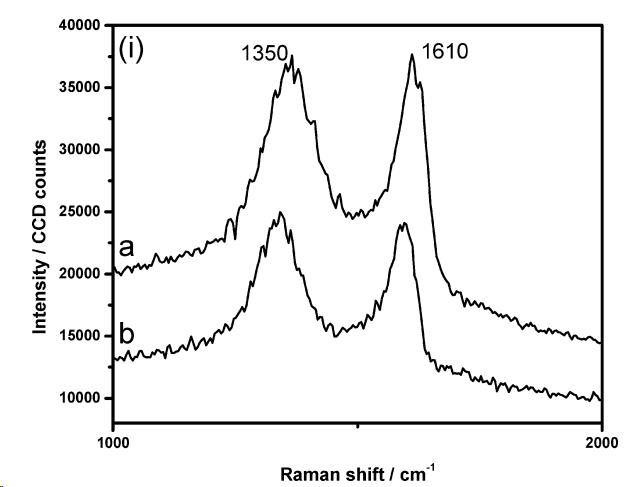
\includegraphics[scale=0.4]{img/Raman}
    \caption{拉曼光谱图。a线为氧化石墨烯,b线为电化学还原后的石墨烯。}
\end{figure}


\subsection{红外光谱(IR)表征}

IR的主要用途是定性表征石墨烯及其衍生物和复合材料的结构。通过观察吸收峰,可以获得有关官能团的信息,从而进一步分析材料的结构。

我们用氧化石墨烯的电化学还原作为例子。如图~\ref{fig:IR}所示,还原后得到的EGS与还原前的EGO的吸收峰强度有明显不同,这能够说明电化学还原的有效进行\cite{RN32}。

\begin{figure}
    \centering
    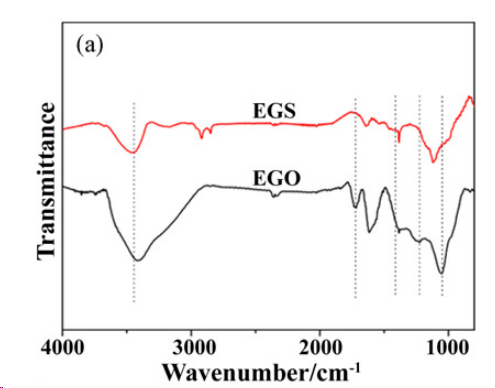
\includegraphics[scale=0.4]{img/IR}
    \caption{EGO与EGS的IR图像}
    \label{fig:IR}
\end{figure}


\subsection{X射线光电子能谱(XPS)表征}

XPS可分析官能团并对各种官能团做含量计算,因此可用于石墨烯及其衍生物或复合材料中化学结构和化学组分的定性及定量表征。



\subsection{紫外光谱(UV)表征}

UV表征常用于定性分析,通过图像的对比,大致判断产物是否为石墨烯或其衍生物。

UV可以用于表征氧化石墨烯的还原过程,下图展示了图像随还原时间的变化\cite{RN33}:

\begin{figure}
    \centering
    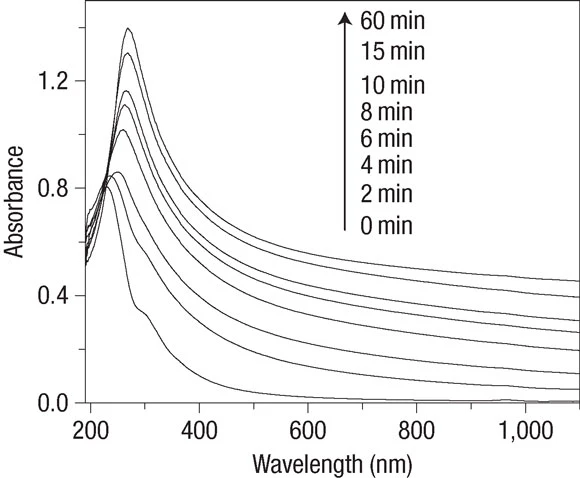
\includegraphics[scale=0.4]{img/UV}
    \caption{氧化石墨烯还原过程的UV图像}
\end{figure}